\chapter{System Model and Problem Formulation}\label{chap:systemModel}

In this chapter, we introduce the system model of a Multi-Radio Cognitive Radio Network (MRCRN). Additionally, we list down several assumptions for the system model. For this system model, we then define our research problem.

\section{System Model}

We consider a cognitive radio network (as described in Figure~\ref{fig:systemmodel}) having $n$ primary users and $m$ secondary users in our analysis. For the sake of simplicity, we assume that $n$ primary users use $n$ distinct spectrum channels. Primary users randomly become active and inactive in their respective channel following a Poisson process~\cite{Ross}. Dedicated single PU for a single channel can actually model multiple PUs per channel. Also, when PU becomes active, SUs' transmission is held back instantly. Therefore, PUs do not refrain from using their dedicated channel.

Each of the $m$ secondary users has at least $2$ radios. Here, one radio is for control purpose, and remaining ones are for data communication and channel sensing activities. There is a dedicated control channel for the control radios, which we assume not to be used by any of the primary users. For control channel, recent studies~\cite{ACH, lo2011survey, thilina2016dccc} have proposed several strategies to establish a control channel via channel hopping when there is no PU free channel in the system model. Therefore, we can assume such methods can be adopted to establish a control channel for our system model when no primary user free channel is available. 

This dedicated control channel is utilized into time slots. Each time slot has $m$ sub-slots, one for each of the secondary users. In each sub-slot, the respective secondary user's control radio transmits its current communication parameters to avoid hidden terminal and synchronization problems. We assume that there is no inter-channel interference among the data channels. Also, we only consider single-hop data communication for secondary users.

\begin{figure}[!htb]
\begin{center}
\begin{tikzpicture}[scale=0.5, transform shape]
    \node {\begin{tikzpicture}[scale=2.0, transform shape]
    %\draw [help lines] (0, 0) grid (10, 7);
    \draw (0, 0) node {\begin{tikzpicture}[scale=1.0, transform shape]
    \node[draw=white, thick] (puRadio) {
        \begin{tikzpicture} [scale=0.5]
        \draw [line width=0.25mm, bend right = 15, red] (2, -0.44) to (2.5,0.44);
        \draw [line width=0.25mm, bend left = 15, red] (3, -0.44) to (2.5,0.44);
        \draw [line width=0.25mm, red] (2.15, -0.3) to (2.85,-0.3);
        \draw [line width=0.25mm, red] (2.25, -0.15) to (2.75,-0.15);
        \draw [line width=0.25mm, red] (2.35, 0) to (2.65,0);
        %\draw [line width=0.25mm] (2.5, -0.44) to (2.5,0.44);
        \draw [fill=red, red] (2.5,0.44) circle(1.5mm);

        \draw [line width=0.25mm, red] (2.5, 0.725) to (2.5,1.0);
        \draw [line width=0.25mm, red] (2.65, 0.65) to (2.825,0.85);
        \draw [line width=0.25mm, red] (2.725, 0.44) to (3,0.44);
        \draw [line width=0.25mm, red] (2.35, 0.65) to (2.175,0.85);
        \draw [line width=0.25mm, red] (2.275, 0.44) to (2,0.44);

        \end{tikzpicture}
    };
\end{tikzpicture}};
    \draw (0, -1) node {\LARGE PU$_{n-1}$};
    
    \draw [fill=red!100!black, red!100!black] (0,3.5) circle(0.5mm);
    \draw [fill=red!100!black, red!100!black] (0,3) circle(0.5mm);
    \draw [fill=red!100!black, red!100!black] (0,2.5) circle(0.5mm);
    
    \draw (0, 7) node {\begin{tikzpicture}[scale=1.0, transform shape]
    \node[draw=white, thick] (puRadio) {
        \begin{tikzpicture} [scale=0.5]
        \draw [line width=0.25mm, bend right = 15, red] (2, -0.44) to (2.5,0.44);
        \draw [line width=0.25mm, bend left = 15, red] (3, -0.44) to (2.5,0.44);
        \draw [line width=0.25mm, red] (2.15, -0.3) to (2.85,-0.3);
        \draw [line width=0.25mm, red] (2.25, -0.15) to (2.75,-0.15);
        \draw [line width=0.25mm, red] (2.35, 0) to (2.65,0);
        %\draw [line width=0.25mm] (2.5, -0.44) to (2.5,0.44);
        \draw [fill=red, red] (2.5,0.44) circle(1.5mm);

        \draw [line width=0.25mm, red] (2.5, 0.725) to (2.5,1.0);
        \draw [line width=0.25mm, red] (2.65, 0.65) to (2.825,0.85);
        \draw [line width=0.25mm, red] (2.725, 0.44) to (3,0.44);
        \draw [line width=0.25mm, red] (2.35, 0.65) to (2.175,0.85);
        \draw [line width=0.25mm, red] (2.275, 0.44) to (2,0.44);

        \end{tikzpicture}
    };
\end{tikzpicture}};
    \draw (0, 6) node {\LARGE PU$_1$};
    \draw (10, 7) node {\begin{tikzpicture}[scale=1.0, transform shape]
    \node[draw=white, thick] (puRadio) {
        \begin{tikzpicture} [scale=0.5]
        \draw [line width=0.25mm, bend right = 15, red] (2, -0.44) to (2.5,0.44);
        \draw [line width=0.25mm, bend left = 15, red] (3, -0.44) to (2.5,0.44);
        \draw [line width=0.25mm, red] (2.15, -0.3) to (2.85,-0.3);
        \draw [line width=0.25mm, red] (2.25, -0.15) to (2.75,-0.15);
        \draw [line width=0.25mm, red] (2.35, 0) to (2.65,0);
        %\draw [line width=0.25mm] (2.5, -0.44) to (2.5,0.44);
        \draw [fill=red, red] (2.5,0.44) circle(1.5mm);

        \draw [line width=0.25mm, red] (2.5, 0.725) to (2.5,1.0);
        \draw [line width=0.25mm, red] (2.65, 0.65) to (2.825,0.85);
        \draw [line width=0.25mm, red] (2.725, 0.44) to (3,0.44);
        \draw [line width=0.25mm, red] (2.35, 0.65) to (2.175,0.85);
        \draw [line width=0.25mm, red] (2.275, 0.44) to (2,0.44);

        \end{tikzpicture}
    };
\end{tikzpicture}};
    \draw (10, 6) node {\LARGE PU$_2$};
    
    \draw [fill=red!100!black, red!100!black] (10,3.5) circle(0.5mm);
    \draw [fill=red!100!black, red!100!black] (10,3) circle(0.5mm);
    \draw [fill=red!100!black, red!100!black] (10,2.5) circle(0.5mm);
    
    \draw (10, 0) node {\begin{tikzpicture}[scale=1.0, transform shape]
    \node[draw=white, thick] (puRadio) {
        \begin{tikzpicture} [scale=0.5]
        \draw [line width=0.25mm, bend right = 15, red] (2, -0.44) to (2.5,0.44);
        \draw [line width=0.25mm, bend left = 15, red] (3, -0.44) to (2.5,0.44);
        \draw [line width=0.25mm, red] (2.15, -0.3) to (2.85,-0.3);
        \draw [line width=0.25mm, red] (2.25, -0.15) to (2.75,-0.15);
        \draw [line width=0.25mm, red] (2.35, 0) to (2.65,0);
        %\draw [line width=0.25mm] (2.5, -0.44) to (2.5,0.44);
        \draw [fill=red, red] (2.5,0.44) circle(1.5mm);

        \draw [line width=0.25mm, red] (2.5, 0.725) to (2.5,1.0);
        \draw [line width=0.25mm, red] (2.65, 0.65) to (2.825,0.85);
        \draw [line width=0.25mm, red] (2.725, 0.44) to (3,0.44);
        \draw [line width=0.25mm, red] (2.35, 0.65) to (2.175,0.85);
        \draw [line width=0.25mm, red] (2.275, 0.44) to (2,0.44);

        \end{tikzpicture}
    };
\end{tikzpicture}};
    \draw (10, -1) node {\LARGE PU$_n$};
    %\draw [fill=green!50!white] (-2, -2) rectangle (2, -1);
    
    \draw (5, 6.7) node {\begin{tikzpicture}[scale=0.375, transform shape]
    \node (controlRadio)
    {
        \begin{tikzpicture} [scale=1.0]
        \draw [fill=blue!25!white, blue!75!black] (2.3, -0.44) -- (2.5,0.44) -- (2.7, -0.44);
        \draw [fill=blue!25!white, blue!75!black] (2.5,0.44) circle(1.5mm);

        \draw [line width=0.25mm, blue!25!white] (2.5, 0.725) to (2.5,1.0);
        \draw [line width=0.25mm, blue!25!white] (2.65, 0.65) to (2.825,0.85);
        \draw [line width=0.25mm, blue!25!white] (2.725, 0.44) to (3,0.44);
        \draw [line width=0.25mm, blue!25!white] (2.35, 0.65) to (2.175,0.85);
        \draw [line width=0.25mm, blue!25!white] (2.275, 0.44) to (2,0.44);

        \end{tikzpicture}
    };
    \node (dataRadio1) [below=of controlRadio, xshift=-1.0cm, yshift=0.5cm] %, xshift=-1.5mm
    {
        
\begin{tikzpicture} [scale=0.75]
        \draw [line width=0.25mm, green!50!black] (2, -0.44) to (2.5,0.44);
        \draw [line width=0.25mm, green!50!black] (3, -0.44) to (2.5,0.44);
        \draw [line width=0.25mm, green!50!black] (2, -0.44) to (3,-0.44);
        \draw [line width=0.25mm, green!50!black] (2.5, -0.44) to (2.5,0.44);
        \draw [fill=green!50!black, green!50!black] (2.5,0.44) circle(1.5mm);

        \draw [line width=0.25mm, green!50!black] (2.5, 0.725) to (2.5,1.0);
        \draw [line width=0.25mm, green!50!black] (2.65, 0.65) to (2.825,0.85);
        \draw [line width=0.25mm, green!50!black] (2.725, 0.44) to (3,0.44);
        \draw [line width=0.25mm, green!50!black] (2.35, 0.65) to (2.175,0.85);
        \draw [line width=0.25mm, green!50!black] (2.275, 0.44) to (2,0.44);

        \end{tikzpicture}
    };
    %()
    \draw[fill=green!50!black, green!50!black] (-0.25,-2.15) circle (0.025);
    \draw[fill=green!50!black, green!50!black] (0,-2.15) circle (0.025);
    \draw[fill=green!50!black, green!50!black] (0.25,-2.15) circle (0.025);
    %
    \node (dataRadio2) [right=of dataRadio1] %, xshift=-1.5mm
    {
        
\begin{tikzpicture} [scale=0.75]
        \draw [line width=0.25mm, green!50!black] (2, -0.44) to (2.5,0.44);
        \draw [line width=0.25mm, green!50!black] (3, -0.44) to (2.5,0.44);
        \draw [line width=0.25mm, green!50!black] (2, -0.44) to (3,-0.44);
        \draw [line width=0.25mm, green!50!black] (2.5, -0.44) to (2.5,0.44);
        \draw [fill=green!50!black, green!50!black] (2.5,0.44) circle(1.5mm);

        \draw [line width=0.25mm, green!50!black] (2.5, 0.725) to (2.5,1.0);
        \draw [line width=0.25mm, green!50!black] (2.65, 0.65) to (2.825,0.85);
        \draw [line width=0.25mm, green!50!black] (2.725, 0.44) to (3,0.44);
        \draw [line width=0.25mm, green!50!black] (2.35, 0.65) to (2.175,0.85);
        \draw [line width=0.25mm, green!50!black] (2.275, 0.44) to (2,0.44);

        \end{tikzpicture}
    };%fill=green!50!black,
    \draw[line width=0.25mm, green!25!black] (0.25,-1) circle (3);
\end{tikzpicture}
};
    \draw (5, 8.2) node {\LARGE SU$_1$};
    \draw (1.5, 4) node {\begin{tikzpicture}[scale=0.375, transform shape]
    \node (controlRadio)
    {
        \begin{tikzpicture} [scale=1.0]
        \draw [fill=blue!25!white, blue!75!black] (2.3, -0.44) -- (2.5,0.44) -- (2.7, -0.44);
        \draw [fill=blue!25!white, blue!75!black] (2.5,0.44) circle(1.5mm);

        \draw [line width=0.25mm, blue!25!white] (2.5, 0.725) to (2.5,1.0);
        \draw [line width=0.25mm, blue!25!white] (2.65, 0.65) to (2.825,0.85);
        \draw [line width=0.25mm, blue!25!white] (2.725, 0.44) to (3,0.44);
        \draw [line width=0.25mm, blue!25!white] (2.35, 0.65) to (2.175,0.85);
        \draw [line width=0.25mm, blue!25!white] (2.275, 0.44) to (2,0.44);

        \end{tikzpicture}
    };
    \node (dataRadio1) [below=of controlRadio, xshift=-1.0cm, yshift=0.5cm] %, xshift=-1.5mm
    {
        
\begin{tikzpicture} [scale=0.75]
        \draw [line width=0.25mm, green!50!black] (2, -0.44) to (2.5,0.44);
        \draw [line width=0.25mm, green!50!black] (3, -0.44) to (2.5,0.44);
        \draw [line width=0.25mm, green!50!black] (2, -0.44) to (3,-0.44);
        \draw [line width=0.25mm, green!50!black] (2.5, -0.44) to (2.5,0.44);
        \draw [fill=green!50!black, green!50!black] (2.5,0.44) circle(1.5mm);

        \draw [line width=0.25mm, green!50!black] (2.5, 0.725) to (2.5,1.0);
        \draw [line width=0.25mm, green!50!black] (2.65, 0.65) to (2.825,0.85);
        \draw [line width=0.25mm, green!50!black] (2.725, 0.44) to (3,0.44);
        \draw [line width=0.25mm, green!50!black] (2.35, 0.65) to (2.175,0.85);
        \draw [line width=0.25mm, green!50!black] (2.275, 0.44) to (2,0.44);

        \end{tikzpicture}
    };
    %()
    \draw[fill=green!50!black, green!50!black] (-0.25,-2.15) circle (0.025);
    \draw[fill=green!50!black, green!50!black] (0,-2.15) circle (0.025);
    \draw[fill=green!50!black, green!50!black] (0.25,-2.15) circle (0.025);
    %
    \node (dataRadio2) [right=of dataRadio1] %, xshift=-1.5mm
    {
        
\begin{tikzpicture} [scale=0.75]
        \draw [line width=0.25mm, green!50!black] (2, -0.44) to (2.5,0.44);
        \draw [line width=0.25mm, green!50!black] (3, -0.44) to (2.5,0.44);
        \draw [line width=0.25mm, green!50!black] (2, -0.44) to (3,-0.44);
        \draw [line width=0.25mm, green!50!black] (2.5, -0.44) to (2.5,0.44);
        \draw [fill=green!50!black, green!50!black] (2.5,0.44) circle(1.5mm);

        \draw [line width=0.25mm, green!50!black] (2.5, 0.725) to (2.5,1.0);
        \draw [line width=0.25mm, green!50!black] (2.65, 0.65) to (2.825,0.85);
        \draw [line width=0.25mm, green!50!black] (2.725, 0.44) to (3,0.44);
        \draw [line width=0.25mm, green!50!black] (2.35, 0.65) to (2.175,0.85);
        \draw [line width=0.25mm, green!50!black] (2.275, 0.44) to (2,0.44);

        \end{tikzpicture}
    };%fill=green!50!black,
    \draw[line width=0.25mm, green!25!black] (0.25,-1) circle (3);
\end{tikzpicture}
};
    \draw (1.55, 5.5) node {\LARGE SU$_2$};
    
    \draw [fill=green!50!black, green!50!black] (1.25,2.65) circle(0.5mm);
    \draw [fill=green!50!black, green!50!black] (1.5,2.4) circle(0.5mm);
    \draw [fill=green!50!black, green!50!black] (1.75,2.15) circle(0.5mm);
    
    \draw (2.5, 1) node {\begin{tikzpicture}[scale=0.375, transform shape]
    \node (controlRadio)
    {
        \begin{tikzpicture} [scale=1.0]
        \draw [fill=blue!25!white, blue!75!black] (2.3, -0.44) -- (2.5,0.44) -- (2.7, -0.44);
        \draw [fill=blue!25!white, blue!75!black] (2.5,0.44) circle(1.5mm);

        \draw [line width=0.25mm, blue!25!white] (2.5, 0.725) to (2.5,1.0);
        \draw [line width=0.25mm, blue!25!white] (2.65, 0.65) to (2.825,0.85);
        \draw [line width=0.25mm, blue!25!white] (2.725, 0.44) to (3,0.44);
        \draw [line width=0.25mm, blue!25!white] (2.35, 0.65) to (2.175,0.85);
        \draw [line width=0.25mm, blue!25!white] (2.275, 0.44) to (2,0.44);

        \end{tikzpicture}
    };
    \node (dataRadio1) [below=of controlRadio, xshift=-1.0cm, yshift=0.5cm] %, xshift=-1.5mm
    {
        
\begin{tikzpicture} [scale=0.75]
        \draw [line width=0.25mm, green!50!black] (2, -0.44) to (2.5,0.44);
        \draw [line width=0.25mm, green!50!black] (3, -0.44) to (2.5,0.44);
        \draw [line width=0.25mm, green!50!black] (2, -0.44) to (3,-0.44);
        \draw [line width=0.25mm, green!50!black] (2.5, -0.44) to (2.5,0.44);
        \draw [fill=green!50!black, green!50!black] (2.5,0.44) circle(1.5mm);

        \draw [line width=0.25mm, green!50!black] (2.5, 0.725) to (2.5,1.0);
        \draw [line width=0.25mm, green!50!black] (2.65, 0.65) to (2.825,0.85);
        \draw [line width=0.25mm, green!50!black] (2.725, 0.44) to (3,0.44);
        \draw [line width=0.25mm, green!50!black] (2.35, 0.65) to (2.175,0.85);
        \draw [line width=0.25mm, green!50!black] (2.275, 0.44) to (2,0.44);

        \end{tikzpicture}
    };
    %()
    \draw[fill=green!50!black, green!50!black] (-0.25,-2.15) circle (0.025);
    \draw[fill=green!50!black, green!50!black] (0,-2.15) circle (0.025);
    \draw[fill=green!50!black, green!50!black] (0.25,-2.15) circle (0.025);
    %
    \node (dataRadio2) [right=of dataRadio1] %, xshift=-1.5mm
    {
        
\begin{tikzpicture} [scale=0.75]
        \draw [line width=0.25mm, green!50!black] (2, -0.44) to (2.5,0.44);
        \draw [line width=0.25mm, green!50!black] (3, -0.44) to (2.5,0.44);
        \draw [line width=0.25mm, green!50!black] (2, -0.44) to (3,-0.44);
        \draw [line width=0.25mm, green!50!black] (2.5, -0.44) to (2.5,0.44);
        \draw [fill=green!50!black, green!50!black] (2.5,0.44) circle(1.5mm);

        \draw [line width=0.25mm, green!50!black] (2.5, 0.725) to (2.5,1.0);
        \draw [line width=0.25mm, green!50!black] (2.65, 0.65) to (2.825,0.85);
        \draw [line width=0.25mm, green!50!black] (2.725, 0.44) to (3,0.44);
        \draw [line width=0.25mm, green!50!black] (2.35, 0.65) to (2.175,0.85);
        \draw [line width=0.25mm, green!50!black] (2.275, 0.44) to (2,0.44);

        \end{tikzpicture}
    };%fill=green!50!black,
    \draw[line width=0.25mm, green!25!black] (0.25,-1) circle (3);
\end{tikzpicture}
};
    \draw (2.5, 2.5) node {\LARGE SU$_{m-1}$};
    \draw (7.5, 1) node {\begin{tikzpicture}[scale=0.375, transform shape]
    \node (controlRadio)
    {
        \begin{tikzpicture} [scale=1.0]
        \draw [fill=blue!25!white, blue!75!black] (2.3, -0.44) -- (2.5,0.44) -- (2.7, -0.44);
        \draw [fill=blue!25!white, blue!75!black] (2.5,0.44) circle(1.5mm);

        \draw [line width=0.25mm, blue!25!white] (2.5, 0.725) to (2.5,1.0);
        \draw [line width=0.25mm, blue!25!white] (2.65, 0.65) to (2.825,0.85);
        \draw [line width=0.25mm, blue!25!white] (2.725, 0.44) to (3,0.44);
        \draw [line width=0.25mm, blue!25!white] (2.35, 0.65) to (2.175,0.85);
        \draw [line width=0.25mm, blue!25!white] (2.275, 0.44) to (2,0.44);

        \end{tikzpicture}
    };
    \node (dataRadio1) [below=of controlRadio, xshift=-1.0cm, yshift=0.5cm] %, xshift=-1.5mm
    {
        
\begin{tikzpicture} [scale=0.75]
        \draw [line width=0.25mm, green!50!black] (2, -0.44) to (2.5,0.44);
        \draw [line width=0.25mm, green!50!black] (3, -0.44) to (2.5,0.44);
        \draw [line width=0.25mm, green!50!black] (2, -0.44) to (3,-0.44);
        \draw [line width=0.25mm, green!50!black] (2.5, -0.44) to (2.5,0.44);
        \draw [fill=green!50!black, green!50!black] (2.5,0.44) circle(1.5mm);

        \draw [line width=0.25mm, green!50!black] (2.5, 0.725) to (2.5,1.0);
        \draw [line width=0.25mm, green!50!black] (2.65, 0.65) to (2.825,0.85);
        \draw [line width=0.25mm, green!50!black] (2.725, 0.44) to (3,0.44);
        \draw [line width=0.25mm, green!50!black] (2.35, 0.65) to (2.175,0.85);
        \draw [line width=0.25mm, green!50!black] (2.275, 0.44) to (2,0.44);

        \end{tikzpicture}
    };
    %()
    \draw[fill=green!50!black, green!50!black] (-0.25,-2.15) circle (0.025);
    \draw[fill=green!50!black, green!50!black] (0,-2.15) circle (0.025);
    \draw[fill=green!50!black, green!50!black] (0.25,-2.15) circle (0.025);
    %
    \node (dataRadio2) [right=of dataRadio1] %, xshift=-1.5mm
    {
        
\begin{tikzpicture} [scale=0.75]
        \draw [line width=0.25mm, green!50!black] (2, -0.44) to (2.5,0.44);
        \draw [line width=0.25mm, green!50!black] (3, -0.44) to (2.5,0.44);
        \draw [line width=0.25mm, green!50!black] (2, -0.44) to (3,-0.44);
        \draw [line width=0.25mm, green!50!black] (2.5, -0.44) to (2.5,0.44);
        \draw [fill=green!50!black, green!50!black] (2.5,0.44) circle(1.5mm);

        \draw [line width=0.25mm, green!50!black] (2.5, 0.725) to (2.5,1.0);
        \draw [line width=0.25mm, green!50!black] (2.65, 0.65) to (2.825,0.85);
        \draw [line width=0.25mm, green!50!black] (2.725, 0.44) to (3,0.44);
        \draw [line width=0.25mm, green!50!black] (2.35, 0.65) to (2.175,0.85);
        \draw [line width=0.25mm, green!50!black] (2.275, 0.44) to (2,0.44);

        \end{tikzpicture}
    };%fill=green!50!black,
    \draw[line width=0.25mm, green!25!black] (0.25,-1) circle (3);
\end{tikzpicture}
};
    \draw (7.5, 2.5) node {\LARGE SU$_m$};
    
    \draw [fill=green!50!black, green!50!black] (8.6,2.65) circle(0.5mm);
    \draw [fill=green!50!black, green!50!black] (8.35,2.4) circle(0.5mm);
    \draw [fill=green!50!black, green!50!black] (8.1,2.15) circle(0.5mm);
    
    \draw (8.5, 4) node {\begin{tikzpicture}[scale=0.375, transform shape]
    \node (controlRadio)
    {
        \begin{tikzpicture} [scale=1.0]
        \draw [fill=blue!25!white, blue!75!black] (2.3, -0.44) -- (2.5,0.44) -- (2.7, -0.44);
        \draw [fill=blue!25!white, blue!75!black] (2.5,0.44) circle(1.5mm);

        \draw [line width=0.25mm, blue!25!white] (2.5, 0.725) to (2.5,1.0);
        \draw [line width=0.25mm, blue!25!white] (2.65, 0.65) to (2.825,0.85);
        \draw [line width=0.25mm, blue!25!white] (2.725, 0.44) to (3,0.44);
        \draw [line width=0.25mm, blue!25!white] (2.35, 0.65) to (2.175,0.85);
        \draw [line width=0.25mm, blue!25!white] (2.275, 0.44) to (2,0.44);

        \end{tikzpicture}
    };
    \node (dataRadio1) [below=of controlRadio, xshift=-1.0cm, yshift=0.5cm] %, xshift=-1.5mm
    {
        
\begin{tikzpicture} [scale=0.75]
        \draw [line width=0.25mm, green!50!black] (2, -0.44) to (2.5,0.44);
        \draw [line width=0.25mm, green!50!black] (3, -0.44) to (2.5,0.44);
        \draw [line width=0.25mm, green!50!black] (2, -0.44) to (3,-0.44);
        \draw [line width=0.25mm, green!50!black] (2.5, -0.44) to (2.5,0.44);
        \draw [fill=green!50!black, green!50!black] (2.5,0.44) circle(1.5mm);

        \draw [line width=0.25mm, green!50!black] (2.5, 0.725) to (2.5,1.0);
        \draw [line width=0.25mm, green!50!black] (2.65, 0.65) to (2.825,0.85);
        \draw [line width=0.25mm, green!50!black] (2.725, 0.44) to (3,0.44);
        \draw [line width=0.25mm, green!50!black] (2.35, 0.65) to (2.175,0.85);
        \draw [line width=0.25mm, green!50!black] (2.275, 0.44) to (2,0.44);

        \end{tikzpicture}
    };
    %()
    \draw[fill=green!50!black, green!50!black] (-0.25,-2.15) circle (0.025);
    \draw[fill=green!50!black, green!50!black] (0,-2.15) circle (0.025);
    \draw[fill=green!50!black, green!50!black] (0.25,-2.15) circle (0.025);
    %
    \node (dataRadio2) [right=of dataRadio1] %, xshift=-1.5mm
    {
        
\begin{tikzpicture} [scale=0.75]
        \draw [line width=0.25mm, green!50!black] (2, -0.44) to (2.5,0.44);
        \draw [line width=0.25mm, green!50!black] (3, -0.44) to (2.5,0.44);
        \draw [line width=0.25mm, green!50!black] (2, -0.44) to (3,-0.44);
        \draw [line width=0.25mm, green!50!black] (2.5, -0.44) to (2.5,0.44);
        \draw [fill=green!50!black, green!50!black] (2.5,0.44) circle(1.5mm);

        \draw [line width=0.25mm, green!50!black] (2.5, 0.725) to (2.5,1.0);
        \draw [line width=0.25mm, green!50!black] (2.65, 0.65) to (2.825,0.85);
        \draw [line width=0.25mm, green!50!black] (2.725, 0.44) to (3,0.44);
        \draw [line width=0.25mm, green!50!black] (2.35, 0.65) to (2.175,0.85);
        \draw [line width=0.25mm, green!50!black] (2.275, 0.44) to (2,0.44);

        \end{tikzpicture}
    };%fill=green!50!black,
    \draw[line width=0.25mm, green!25!black] (0.25,-1) circle (3);
\end{tikzpicture}
};
    \draw (8.5, 5.5) node {\LARGE SU$_3$};
    
    \draw (5, 4.9) node {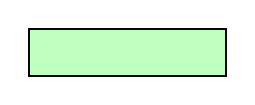
\begin{tikzpicture}[scale=1.0, transform shape]
    \tikzstyle{every node} = [draw, shape = rectangle, node distance=0mm, minimum width=4mm, minimum height=6mm, fill=green!25!white]
    \node[draw=black, thick, minimum width=25mm] (channel1) {};
\end{tikzpicture}
};
    \draw (5, 4.2) node {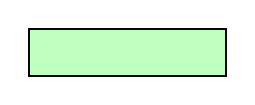
\begin{tikzpicture}[scale=1.0, transform shape]
    \tikzstyle{every node} = [draw, shape = rectangle, node distance=0mm, minimum width=4mm, minimum height=6mm, fill=green!25!white]
    \node[draw=black, thick, minimum width=25mm] (channel1) {};
\end{tikzpicture}
};
    \draw (5, 3.5) node {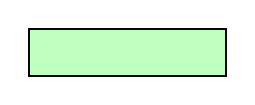
\begin{tikzpicture}[scale=1.0, transform shape]
    \tikzstyle{every node} = [draw, shape = rectangle, node distance=0mm, minimum width=4mm, minimum height=6mm, fill=green!25!white]
    \node[draw=black, thick, minimum width=25mm] (channel1) {};
\end{tikzpicture}
};
    \draw (5, 2.8) node {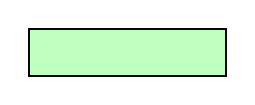
\begin{tikzpicture}[scale=1.0, transform shape]
    \tikzstyle{every node} = [draw, shape = rectangle, node distance=0mm, minimum width=4mm, minimum height=6mm, fill=green!25!white]
    \node[draw=black, thick, minimum width=25mm] (channel1) {};
\end{tikzpicture}
};%[label=above:{\LARGE \(n\) spectrum channels}]
    \draw (5, 2.1) node {\LARGE Channels};
    \draw (5, 1.25) node {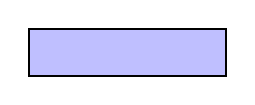
\begin{tikzpicture}[scale=1.0, transform shape]
    \tikzstyle{every node} = [draw, shape = rectangle, node distance=0mm, minimum width=4mm, minimum height=6mm, fill=blue!25!white]
    \node[draw=black, thick, minimum width=25mm] (channel1) {};
\end{tikzpicture}
};%[label=below:{\LARGE dedicated control channel}]
    \draw (5, 0.5) node {\LARGE Control};
    \draw (5, -0.15) node {\LARGE channel};

\end{tikzpicture}
};
\end{tikzpicture}
\caption{System model of a MRCRN}
\label{fig:systemmodel}
\end{center}
\vspace{-1cm}
\end{figure}

\section{Problem Definition}

Under the presented system model, our research question is how to efficiently use the available multiple data transmission radios to get enhanced total network throughput while limiting end-to-end delay. As there is no central authority in the considered system model, solution of the problem must be distributed. Besides, the decision making must also be online as the primary and secondary users' behavior can dynamically vary and thus can not be predicted beforehand. Considering these aspects, we propose a new solution in the next chapter.
\endinput
